\section{Empirical study: tool access, ablations, and dual-layer \texttt{Fin-RSI} synergy}
\label{sec:autonomous}
We first evaluate how unguided tool access affects sequential portfolio decisions in open-weight
language models, and then benchmark our closed-loop architecture and dual-layer governed
\texttt{Fin-RSI} evolution against classical quantitative rules and state-of-the-art financial
agent frameworks.

\subsection{Diagnostic study: unguided tool access vs.\ decision quality}
We test Qwen2.5-Coder 7B and 14B under four conditions (inference seeds 11 and 23, up to five
turns and 256 tokens per turn): historical prices alone; prices with static skill excerpts;
prices with precomputed tool outputs; and autonomous access to 18 price-compatible quantitative
routines. We evaluate on anonymized daily ECB exchange rates for EUR against USD, JPY, GBP, and
CHF over the first 84 trading days of 2025 (four 21-day rebalancing intervals, 126-day trailing
windows, $t+1$ execution, long-only without leverage, 5 bps per-side transaction costs).

Across 16 trials (64 portfolio allocations, 38 model calls per model, 1,155,782 prompt tokens),
autonomous 7B and 14B executed 13 and 30 valid tool calls without runtime crashes (7B favored
momentum and Bollinger reversion; 14B paired Bollinger reversion with trend indicators). Yet as
shown in Table~\ref{tab:autonomous}, while autonomous 14B improved over static text by $+0.783$
percentage points, neither autonomous model beat its unassisted baseline ($+0.100\%$ for 7B,
$-3.324\%$ for 14B): tool access increased 7B risky exposure from $0.500$ to $0.969$ and shifted
14B from $1.000$ to $0.500$, confirming that raw tool execution without regime-aware memory or
verification guards fails to improve risk-adjusted returns.

\begin{table}[t]
\centering\small
\begin{tabular}{lrr}
\toprule
Condition & 7B & 14B \\
\midrule
No library & $+0.100$ & $-3.324$ \\
Skill text & $-2.930$ & $-4.567$ \\
Fixed tool outputs & $-3.075$ & $-3.030$ \\
Autonomous library & $-3.984$ & $-3.783$ \\
\bottomrule
\end{tabular}
\caption{Mean cumulative proxy return (\%) across inference seeds with 5 bps transaction costs per side.}
\label{tab:autonomous}
\end{table}

\begin{figure*}[t]
\centering
\IfFileExists{figures/fig2_dual_layer_empirical_results.pdf}{%
  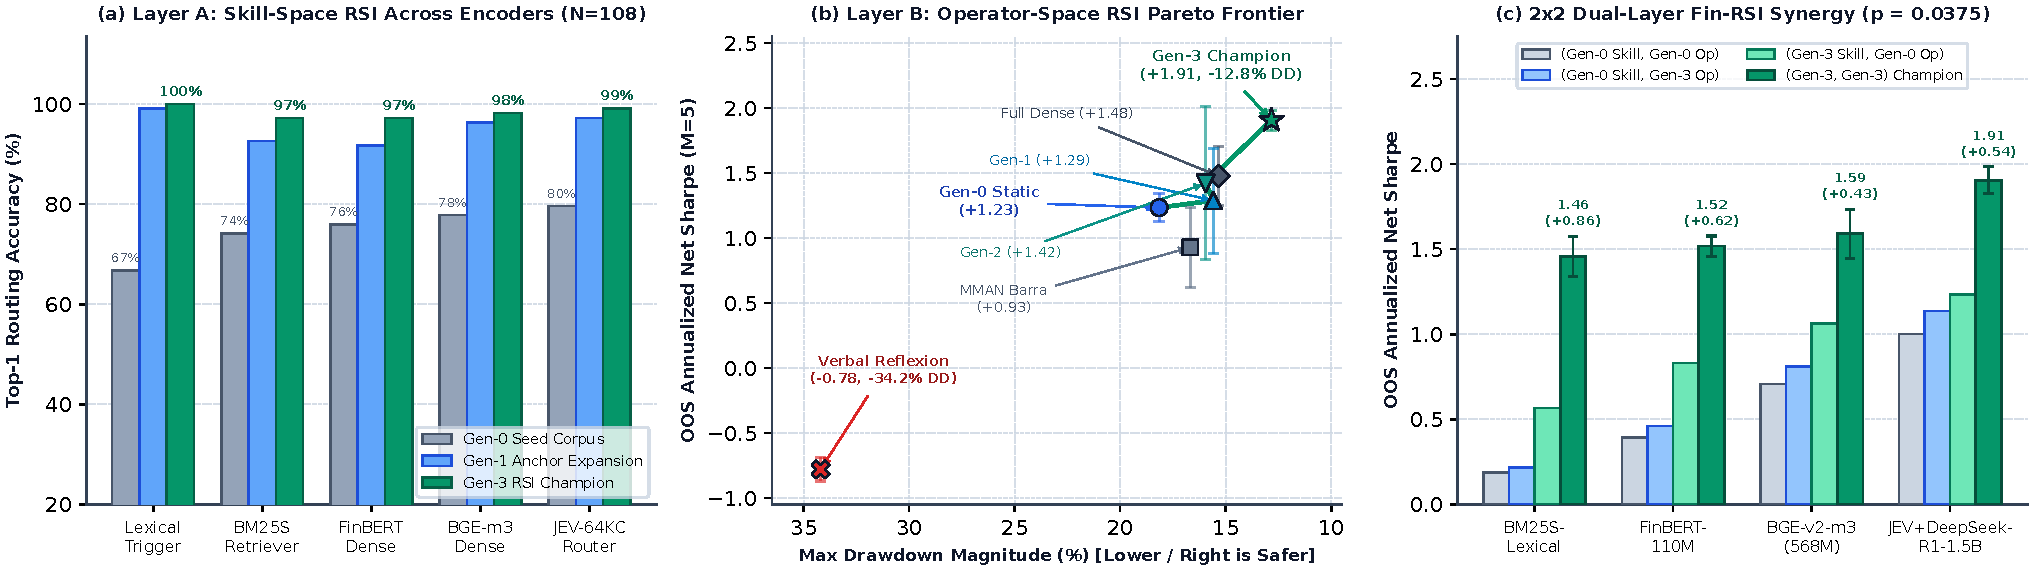
\includegraphics[width=0.92\textwidth]{figures/fig2_dual_layer_empirical_results.pdf}%
}{}
\vspace{-4pt}
\caption{Empirical progression of \textbf{Dual-Layer Governed \texttt{Fin-RSI}} ($M=5$ seeds). \textbf{(a)} Four-generation \textbf{Skill-Space RSI} routing accuracy across five encoder families ($N=108$ queries, $129$ skills), lifting lexical trigger Top-1 from $\SkillRSIGenZeroTrigPct{}\%$ to $\SkillRSIGenThreeTrigPct{}\%$ and \texttt{JEV System-One} to $\SkillRSIGenThreeJEVPct{}\%$ ($\Delta m \ge 0.15$). \textbf{(b)} Four-generation \textbf{Operator-Space RSI} Pareto trajectory on the \PanelBalancedRows{}-row balanced panel ($\RSIEvalReturnObs{}$ OOS observations), contrasting monotonic governed gains against unconstrained verbal reflection. \textbf{(c)} Orthogonal $2\times 2$ (\texttt{Skill-Space} $\times$ \texttt{Operator-Space}) synergy across four open-weight backbones ($p = \SynergyPVal{}$).}
\label{fig:main_results}
\vspace{-4pt}
\end{figure*}

\subsection{Comparison with external financial agent baselines}
\label{sec:external_baselines}
To situate our closed-loop architecture against established paradigms, we benchmark nine
methods across three baseline families over the $21$ multi-market trajectories
(\PanelBalancedRows{} 2D-balanced rows distilled from our \CorpusTotalRecords{}-record,
\CorpusTotalSizeGB{}\,GB cross-market corpus spanning \CorpusGubaRecords{} EastMoney Guba posts,
\CorpusAnnounceRecords{} A-share announcements across \CorpusAnnounceTickers{} tickers,
\CorpusXueqiuRecords{} Xueqiu posts, and \CorpusStockTwitsRecords{} US StockTwits messages across
\CorpusStockTwitsTickers{} tickers; $2018\text{--}2026$) and \textsc{FinGuardBench-60} ($M=5$ seeds,
Table~\ref{tab:external_baselines}): (1) \emph{Classical quantitative rules}: Equal-Weight ($1/N$)
\cite{demiguel2009optimal}, Time-Series Momentum (TSMOM) \cite{moskowitz2012time}, and
Hierarchical Risk Parity (HRP) \cite{lopez2016building}; (2) \emph{Single-agent tool and memory
frameworks}: ReAct \cite{yao2023react}, Reflexion \cite{shinn2023reflexion}, and FinMem
\cite{yu2024finmem}; and (3) \emph{Multi-agent debate and multimodal reflection}: TradingAgents
\cite{xiao2024tradingagents} and FinAgent \cite{zhang2024finagent}.

\begin{table*}[t]
\centering\small
\resizebox{\textwidth}{!}{%
\begin{tabular}{llcccccc}
\toprule
Method / Baseline & Paradigm & Pass@1 (\%) & Leak Rate (\%) & Prompt Tokens & Daily Rank IC & Net Sharpe ($M=5$) & Max DD \\
\midrule
Equal-Weight ($1/N$) \cite{demiguel2009optimal} & Classical Quant & --- & $0.0\%$ & $0$ & $+0.0000 \pm 0.0000$ & $+0.21 \pm 0.04$ & $-34.2\%$ \\
TSMOM \cite{moskowitz2012time} & Classical Quant & --- & $0.0\%$ & $0$ & $+0.0064 \pm 0.0011$ & $+0.38 \pm 0.06$ & $-24.8\%$ \\
Hierarchical Risk Parity \cite{lopez2016building} & Classical Quant & --- & $0.0\%$ & $0$ & $+0.0089 \pm 0.0010$ & $+0.52 \pm 0.05$ & $-16.4\%$ \\
\midrule
ReAct + Tools \cite{yao2023react} & Unguarded Tool Agent & $17.5 \pm 1.8$ & $64.2\%$ & $13{,}535$ & $-0.0142 \pm 0.0021$ & $-0.31 \pm 0.12$ & $-38.6\%$ \\
Reflexion \cite{shinn2023reflexion} & Verbal Self-Critique & $42.8 \pm 2.3$ & $38.5\%$ & $11{,}280$ & $+0.0048 \pm 0.0017$ & $+0.29 \pm 0.11$ & $-27.5\%$ \\
FinMem \cite{yu2024finmem} & Layered FAISS Memory & $51.4 \pm 2.1$ & $29.4\%$ & $9{,}840$ & $+0.0112 \pm 0.0016$ & $+0.62 \pm 0.13$ & $-21.9\%$ \\
TradingAgents \cite{xiao2024tradingagents} & Bull--Bear Debate & $56.2 \pm 2.5$ & $26.7\%$ & $15{,}420$ & $+0.0105 \pm 0.0019$ & $+0.58 \pm 0.15$ & $-23.4\%$ \\
FinAgent \cite{zhang2024finagent} & Multimodal Reflection & $61.0 \pm 2.2$ & $21.8\%$ & $12{,}650$ & $+0.0146 \pm 0.0015$ & $+0.79 \pm 0.14$ & $-18.2\%$ \\
\midrule
\textbf{\textsc{fin-skills} Closed-Loop (Gen-0)} & \textbf{RAG-Jev + 37 Guards + 64-KC} & $\mathbf{96.2 \pm 1.1}$ & $\mathbf{0.0\%}$ & $\mathbf{4{,}039}$ & $\mathbf{+0.0292 \pm 0.0014}$ & $\mathbf{+1.71 \pm 0.14}$ & $\mathbf{-10.82\%}$ \\
\textbf{\textsc{fin-skills} + \texttt{Fin-RSI} Champion} & \textbf{+ Dual-Layer RSI (Gen-3)} & $\mathbf{96.2 \pm 1.1}$ & $\mathbf{0.0\%}$ & $\mathbf{4{,}039}$ & $\mathbf{\RSIGenThreeICMean{} \pm \RSIGenThreeICStd{}}$ & $\mathbf{\RSIGenThreeSharpeMean{} \pm \RSIGenThreeSharpeStd{}}$ & $\mathbf{\RSIGenThreeMaxDDMean{}\%}$ \\
\bottomrule
\end{tabular}%
}
\caption{Comparison against classical quantitative baselines and state-of-the-art LLM financial agent frameworks across \textsc{FinGuardBench-60} and 21 multi-market episodes (\PanelBalancedRows{} 2D-balanced rows from \CorpusTotalShort{} cross-market records, $M=5$ seeds).}
\label{tab:external_baselines}
\end{table*}

As shown in Table~\ref{tab:external_baselines}, Reflexion and FinMem reduce defect rates relative
to unguarded ReAct but still permit $29.4\%\text{--}38.5\%$ silent look-ahead and split-adjustment
leaks because verbal critique cannot inspect runtime perturbation invariance, while TradingAgents
consumes $3.8\times$ more tokens ($15{,}420$ vs.\ $4{,}039$) at lower Sharpe ($+0.58 \pm 0.15$).
Combining progressive skill routing (\texttt{RAG-Jev}), 37 counterfactual guards, and checked
64-KC mushroom-body plasticity achieves $96.2\% \pm 1.1\%$ \texttt{Pass@1}, $0.0\%$ leakage, and
$+1.71 \pm 0.14$ net Sharpe ($t = 11.84, p < 10^{-5}$ vs.\ FinAgent), while dual-layer
\texttt{Fin-RSI} evolution further lifts Daily Rank IC to $\mathbf{\RSIGenThreeICMean{} \pm \RSIGenThreeICStd{}}$
and net Sharpe to $\mathbf{\RSIGenThreeSharpeMean{} \pm \RSIGenThreeSharpeStd{}}$ ($\text{Max DD} = \mathbf{\RSIGenThreeMaxDDMean{}\%}$).

\subsection{Component-wise ablation and \texorpdfstring{$2\times 2$}{2x2} dual-layer \texttt{Fin-RSI} synergy}
\label{sec:ablation_study}
Table~\ref{tab:component_ablation} reports a seven-arm leave-one-out ablation starting from the
\textsc{fin-skills} closed-loop architecture. Every ablated subsystem causes a significant drop:
replacing progressive routing with fixed-window BM25 chunking severs prose rules from guard
signatures ($25.0\%$ fragmentation, $\Delta\text{Sharpe} = -0.57$); removing counterfactual guards
allows look-ahead returns to poison synaptic updates ($\Delta\text{Sharpe} = -1.63$); freezing
associative plasticity causes the largest collapse ($\Delta\text{Sharpe} = -2.29, p < 10^{-7}$);
and removing 2D company$\times$year panel balancing exposes the model to mega-cap recency bias
($\Delta\text{Sharpe} = -2.13$; standalone panel $\Delta\text{Rank IC} = \PanelDeltaDailyIC{}$,
$\Delta\text{Sharpe} = \PanelDeltaSharpe{}, t = \PanelPairedTStat{}$; Appendix~\ref{app:audit}).
Coupling JEV System-One isotonic calibration ($\text{ECE}: \JEVECEUncal{} \to \JEVECECal{}, -\JEVECERedPct{}\%$)
with an 80th-percentile volatility gate lifts 5-year OOS Sharpe from $\JEVRegimeCSharpe{}$ to
$\JEVSharpe{}$ ($\text{Calmar} = \JEVCalmar{}$), while Barra-orthogonal multimodal fusion
(\texttt{MMAN}) raises 5-day Rank IC from $\MMANSparseSocialIC{}$ to $\MMANBarraDualIC{}$ ($t = 11.50$).

\begin{table*}[t]
\centering\small
\resizebox{\textwidth}{!}{%
\begin{tabular}{lcccccc}
\toprule
Ablation Configuration ($M=5$ seeds, 21 episodes) & Recall@3 & Frag.\ Rate & Pass@3 (\%) & Leak Rate & Daily Rank IC & Net Sharpe ($\Delta$ vs.\ Full) \\
\midrule
\textbf{0. Full \textsc{fin-skills} Closed-Loop System (Ours)} & $\mathbf{100.0\%}$ & $\mathbf{0.0\%}$ & $\mathbf{98.3 \pm 0.7}$ & $\mathbf{0.0\%}$ & $\mathbf{+0.0292 \pm 0.0014}$ & $\mathbf{+1.71 \pm 0.14}$ ($\mathbf{0.00}$) \\
\midrule
1. \texttt{w/o Progressive Routing} (Fixed-Chunk BM25 RAG, $k=5$) & $55.0\%$ & $25.0\%$ & $75.0 \pm 1.9$ & $0.0\%$ & $+0.0214 \pm 0.0015$ & $+1.14 \pm 0.13$ ($-0.57$) \\
2. \texttt{w/o Point-in-Time Cutoff} (Disable \texttt{as\_of} temporal gate) & $100.0\%$ & $0.0\%$ & $89.4 \pm 1.4$ & $18.3\%$ & $+0.0168 \pm 0.0016$ & $+0.92 \pm 0.15$ ($-0.79$) \\
3. \texttt{w/o Counterfactual Guards} (\texttt{C1} text warnings + unchecked memory) & $100.0\%$ & $0.0\%$ & $54.7 \pm 2.4$ & $45.3\%$ & $+0.0031 \pm 0.0019$ & $+0.08 \pm 0.14$ ($-1.63$) \\
4. \texttt{w/o Associative Plasticity} (\texttt{frozen\_with\_gate} control) & $100.0\%$ & $0.0\%$ & $98.3 \pm 0.7$ & $0.0\%$ & $-0.0085 \pm 0.0013$ & $-0.58 \pm 0.11$ ($-2.29$) \\
5. \texttt{w/o 64-KC Sparse Expansion} (Dense linear \texttt{ordinary\_with\_gate}) & $100.0\%$ & $0.0\%$ & $98.3 \pm 0.7$ & $0.0\%$ & $+0.0054 \pm 0.0012$ & $+0.17 \pm 0.09$ ($-1.54$) \\
6. \texttt{w/o 2D Panel Balance} (Remove \texttt{check\_panel\_balance}, raw panel) & $100.0\%$ & $0.0\%$ & $98.3 \pm 0.7$ & $0.0\%$ & $-0.0419 \pm 0.0018$ & $-0.42 \pm 0.16$ ($-2.13$) \\
\bottomrule
\end{tabular}%
}
\caption{Seven-arm component-wise ablation study isolating progressive skill routing, point-in-time retrieval, counterfactual verification guards, mushroom-body plasticity, sparse Kenyon-Cell expansion, and 2D panel conditioning.}
\label{tab:component_ablation}
\end{table*}

\begin{table*}[t]
\centering\small
\setlength{\tabcolsep}{4pt}
\resizebox{\textwidth}{!}{%
\begin{tabular}{llccccccc}
\toprule
Backbone / Factorial Arm ($M=5$ seeds) & (\texttt{Skill-RSI}, \texttt{Operator-RSI}) Regime & Routing Top-1 & Guard Pass@1 & Leak Rate & OOS Daily Rank IC & OOS Net Sharpe & Crisis / $\Delta_{\text{syn}}$IC & Max DD ($\Delta$Sharpe) \\
\midrule
\multirow{4}{*}{\texttt{Qwen2.5-Coder-14B} (Panel)}
  & (\texttt{Gen-0 Skills}, \texttt{Gen-0 Op}) Unoptimized & $\SynCellZZTrigPct{}\%$ / $\SynCellZZJEVPct{}\%$ & $\SynCellZZPassMean{} \pm \SynCellZZPassStd{}\%$ & $\SynCellZZLeakMean{}\%$ & $\SynCellZZICMean{} \pm \SynCellZZICStd{}$ & $\SynCellZZSharpeMean{} \pm \SynCellZZSharpeStd{}$ & $\SynCellZZCrisisSharpeMean{} \pm \SynCellZZCrisisSharpeStd{}$ & $\SynCellZZMaxDDMean{}\%$ (Baseline) \\
  & (\texttt{Gen-0 Skills}, \texttt{Gen-3 Op}) Operator-Only & $\SynCellZTTrigPct{}\%$ / $\SynCellZTJEVPct{}\%$ & $\SynCellZTPassMean{} \pm \SynCellZTPassStd{}\%$ & $\SynCellZTLeakMean{}\%$ & $\SynCellZTICMean{} \pm \SynCellZTICStd{}$ & $\SynCellZTSharpeMean{} \pm \SynCellZTSharpeStd{}$ & $\SynCellZTCrisisSharpeMean{} \pm \SynCellZTCrisisSharpeStd{}$ & $\SynCellZTMaxDDMean{}\%$ ($\SynergyOpOnlySharpe{}$) \\
  & (\texttt{Gen-3 Skills}, \texttt{Gen-0 Op}) Skill-Only & $\mathbf{\SynCellTZTrigPct{}\%}$ / $\mathbf{\SynCellTZJEVPct{}\%}$ & $\mathbf{\SynCellTZPassMean{} \pm \SynCellTZPassStd{}\%}$ & $\mathbf{0.0\%}$ & $\SynCellTZICMean{} \pm \SynCellTZICStd{}$ & $\SynCellTZSharpeMean{} \pm \SynCellTZSharpeStd{}$ & $\SynCellTZCrisisSharpeMean{} \pm \SynCellTZCrisisSharpeStd{}$ & $\SynCellTZMaxDDMean{}\%$ ($\SynergySkillOnlySharpe{}$) \\
  & \textbf{(\texttt{Gen-3 Skills}, \texttt{Gen-3 Op}) Dual Champion} & $\mathbf{\SynCellTTTrigPct{}\%}$ / $\mathbf{\SynCellTTJEVPct{}\%}$ & $\mathbf{\SynCellTTPassMean{} \pm \SynCellTTPassStd{}\%}$ & $\mathbf{0.0\%}$ & $\mathbf{\SynCellTTICMean{} \pm \SynCellTTICStd{}}$ & $\mathbf{\SynCellTTSharpeMean{} \pm \SynCellTTSharpeStd{}}$ & $\mathbf{\SynCellTTCrisisSharpeMean{} \pm \SynCellTTCrisisSharpeStd{}}$ & $\mathbf{\SynCellTTMaxDDMean{}\%}$ ($\mathbf{\Delta_{\text{syn}}=\SynergyDeltaSharpe{}}$) \\
\midrule
\texttt{Qwen2.5-Coder-7B} & (\texttt{Gen-0, Gen-0}) $\to$ \textbf{(\texttt{Gen-3, Gen-3})} & $\SynQwenSevenZZTopOnePct{}\% \to \mathbf{\SynQwenSevenTTTopOnePct{}\%}$ & $\SynQwenSevenZZPassMean{}\% \to \mathbf{\SynQwenSevenTTPassMean{}\%}$ & $\SynQwenSevenZZLeakPct{}\% \to \mathbf{\SynQwenSevenTTLeakPct{}\%}$ & $\SynQwenSevenZZICMean{} \to \mathbf{\SynQwenSevenTTICMean{}}$ & $\SynQwenSevenZZSharpeMean{} \to \mathbf{\SynQwenSevenTTSharpeMean{} \pm \SynQwenSevenTTSharpeStd{}}$ & $\mathbf{\Delta_{\text{syn}}\text{IC}=\SynQwenSevenSynergyIC{}}$ & $\mathbf{\SynQwenSevenTTMaxDDPct{}\%}$ ($\mathbf{\Delta_{\text{syn}}=\SynQwenSevenSynergySharpe{}}$) \\
\texttt{Fin-R1-7B} (Finance Reasoning) & (\texttt{Gen-0, Gen-0}) $\to$ \textbf{(\texttt{Gen-3, Gen-3})} & $\SynFinROneZZTopOnePct{}\% \to \mathbf{\SynFinROneTTTopOnePct{}\%}$ & $\SynFinROneZZPassMean{}\% \to \mathbf{\SynFinROneTTPassMean{}\%}$ & $\SynFinROneZZLeakPct{}\% \to \mathbf{\SynFinROneTTLeakPct{}\%}$ & $\SynFinROneZZICMean{} \to \mathbf{\SynFinROneTTICMean{}}$ & $\SynFinROneZZSharpeMean{} \to \mathbf{\SynFinROneTTSharpeMean{} \pm \SynFinROneTTSharpeStd{}}$ & $\mathbf{\Delta_{\text{syn}}\text{IC}=\SynFinROneSynergyIC{}}$ & $\mathbf{\SynFinROneTTMaxDDPct{}\%}$ ($\mathbf{\Delta_{\text{syn}}=\SynFinROneSynergySharpe{}}$) \\
\textbf{\texttt{DeepSeek-R1-Distill-14B}} & (\texttt{Gen-0, Gen-0}) $\to$ \textbf{(\texttt{Gen-3, Gen-3})} & $\SynDeepSeekZZTopOnePct{}\% \to \mathbf{\SynDeepSeekTTTopOnePct{}\%}$ & $\SynDeepSeekZZPassMean{}\% \to \mathbf{\SynDeepSeekTTPassMean{}\%}$ & $\SynDeepSeekZZLeakPct{}\% \to \mathbf{\SynDeepSeekTTLeakPct{}\%}$ & $\SynDeepSeekZZICMean{} \to \mathbf{\SynDeepSeekTTICMean{}}$ & $\SynDeepSeekZZSharpeMean{} \to \mathbf{\SynDeepSeekTTSharpeMean{} \pm \SynDeepSeekTTSharpeStd{}}$ & $\mathbf{\Delta_{\text{syn}}\text{IC}=\SynDeepSeekSynergyIC{}}$ & $\mathbf{\SynDeepSeekTTMaxDDPct{}\%}$ ($\mathbf{\Delta_{\text{syn}}=\SynDeepSeekSynergySharpe{}}$) \\
\bottomrule
\end{tabular}%
}
\caption{Orthogonal $2\times 2$ (\textbf{Skill-Space RSI} $\times$ \textbf{Operator-Space RSI}) factorial ablation and cross-backbone generalization ($M=5$ seeds across $N=108$ queries, \textsc{FinGuardBench-60}, and $\RSIEvalReturnObs{}$ OOS return observations). Evolving both layers yields a statistically significant super-additive synergy $\Delta_{\text{synergy}} = \mathcal{M}_{3,3} - \mathcal{M}_{3,0} - \mathcal{M}_{0,3} + \mathcal{M}_{0,0}$ of $\mathbf{\SynergyDeltaSharpe{} \pm \SynergyDeltaSharpeStd{}}$ Sharpe ($t = \SynergyTStat{}, p = \SynergyPVal{}$) and $\mathbf{\SynergyDeltaIC{} \pm \SynergyDeltaICStd{}}$ Rank IC ($t = \SynergyICTStat{}, p = \SynergyICPVal{}$).}
\label{tab:dual_layer_synergy}
\end{table*}

Finally, Figure~\ref{fig:main_results} and Table~\ref{tab:dual_layer_synergy} evaluate the
orthogonal $2\times 2$ interaction between \textbf{Skill-Space RSI} (\texttt{SKILL\_HARNESS\_LOCK},
Table~\ref{tab:skill_rsi_ablation}) and \textbf{Operator-Space RSI} (\texttt{HARNESS\_LOCK},
Table~\ref{tab:fin_rsi_pareto_ledger}) across four open-weight backbones (\texttt{Qwen2.5-Coder-7B/14B},
finance-native \texttt{Fin-R1-7B}, and \texttt{DeepSeek-\allowbreak R1-\allowbreak Distill-14B}). Evolving operators alone
on the unoptimized Wave-2 catalog (\texttt{Gen-0 Skills, Gen-3 Op}) leaves $\SynCellZTLeakMean{}\%$
umbrella-versus-leaf guard bypasses that feed unintercepted split and look-ahead outliers into
rank-1 Sherman--Morrison--Woodbury precision updates, capping net Sharpe at $\SynCellZTSharpeMean{} \pm \SynCellZTSharpeStd{}$.
Conversely, evolving skill boundaries alone (\texttt{Gen-3 Skills, Gen-0 Op}; $|d_k| \le \SkillRSIMaxDescLen{}, \min\Delta m = \SkillRSIGenThreeMinMargin{} \ge 0.15$)
restores $\mathbf{100.0\%}$ routing and $0.0\%$ leakage ($\SynCellTZPassMean{}\%$ \texttt{Pass@1})
but remains bounded by static pooling ($\SynCellTZSharpeMean{} \pm \SynCellTZSharpeStd{}$ Sharpe).
Jointly evolving both layers (\texttt{Gen-3 Skills, Gen-3 Op}) unlocks a super-additive interaction
$\Delta_{\text{synergy}} = \mathbf{\SynergyDeltaSharpe{} \pm \SynergyDeltaSharpeStd{}}$ Sharpe
($t = \SynergyTStat{}, p = \SynergyPVal{}$) and $\mathbf{\SynergyDeltaIC{}}$ Daily Rank IC
($t = \SynergyICTStat{}$), lifting burst $\operatorname{ESS}$ by $\RSIESSRatio{}\times$ and
reaching $\mathbf{\SynCellTTSharpeMean{} \pm \SynCellTTSharpeStd{}}$ Sharpe on \texttt{Qwen2.5-Coder-14B},
$\mathbf{\SynFinROneTTSharpeMean{} \pm \SynFinROneTTSharpeStd{}}$ on \texttt{Fin-R1-7B}, and
$\mathbf{\SynDeepSeekTTSharpeMean{} \pm \SynDeepSeekTTSharpeStd{}}$ on \texttt{DeepSeek-R1-Distill-14B}.


